%%==================================================
%% chapter01.tex for BIT Master Thesis
%% modified by yang yating
%% version: 0.1
%% last update: Dec 25th, 2016
%%==================================================
\chapter{绪论}
\enchapter{Introduction}
\label{chap:intro}
\section{研究背景}
\ensection{Research Background}

近年来,随着云计算技术的快速发展,无服务器计算(Serverless Computing)凭借其"按需分配、自动弹性伸缩、零基础设施运维"的特性,在微服务、事件驱动型应用、数据处理等领域广泛应用。其核心形态函数即服务(Function as a Service, FaaS)通过细粒度函数部署实现了业务逻辑与资源管理的解耦, 首先,它可以帮助应用程序开发人员专注于核心逻辑,并将与基础架构相关的任务(例如自动缩放)留在无服务器平台上。 其次,它采用了具有细粒度付费模式(例如1MS [7])的pay-as-you-go模型,以便用户可以节省未使用的计算资源的成本。 第三,无服务器计算也使云提供商有益于他们可以更有效地管理资源。Serverless的核心思想是将基础设施的管理责任交给云服务提供商,用户无需关心服务器的配置和管理,可以专注于业务逻辑的实现。

然而,在Serverless环境中,如何高效、安全地运行容器化应用仍然是一个亟待解决的关键问题。
但冷启动延迟问题始终是制约其性能的关键瓶颈,尤其在突发请求和高并发场景下更为显著。

传统Serverless平台依赖容器化技术(如Docker)实现资源隔离与执行环境封装。尽管容器较虚拟机轻量,但其底层依赖的Linux控制组(cgroups)机制在资源分配效率上仍存在不足:
(1)cgroups层级结构的资源协商延迟:在高并发场景下,cgroups的CPU、内存等子系统的协同配置效率低下,导致函数实例初始化过程中产生显著调度延迟10;
(2)静态资源预配置的局限性:现有策略难以动态适应函数负载特征,导致资源碎片化与利用率下降,这一问题在突发流量场景下被放大,形成性能与资源效率的矛盾13。

\subsection{Serverless冷启动问题的技术矛盾} 
Serverless架构的核心优势在于其按需分配资源的特性,即函数实例在无请求时缩容至零,而在请求到来时快速启动以处理任务。然而,这种动态伸缩机制带来了显著的冷启动延迟问题。冷启动是指函数实例从零状态到完全就绪所需的时间,主要包括容器初始化、依赖加载、代码执行环境准备等阶段。研究表明,冷启动延迟通常在数百毫秒到数秒之间,这对于实时性要求较高的应用场景(如在线交易、实时数据处理)是不可接受的716。

冷启动问题的根源在于Serverless平台依赖的容器化技术(如Docker)。尽管容器较虚拟机轻量,但其底层依赖的Linux控制组(cgroups)机制在资源分配效率上仍存在不足:
(1)cgroups层级结构的资源协商延迟:在高并发场景下,cgroups的CPU、内存等子系统的协同配置效率低下,导致函数实例初始化过程中产生显著调度延迟;
(2)静态资源预配置的局限性:现有策略难以动态适应函数负载特征,导致资源碎片化与利用率下降,这一问题在突发流量场景下被放大,形成性能与资源效率的矛盾716。

另一方面,现有安全隔离方案(如容器运行时、微虚拟机)虽提供强隔离性,但其引入的上下文切换、内核拦截等开销与Serverless函数的短生命周期特性冲突。近期研究表明,基于**eBPF(Extended Berkeley Packet Filter)**的轻量级内核可编程技术成为突破传统虚拟化架构的新方向612。eBPF通过沙盒化机制允许用户态程序安全执行内核级操作(如网络过滤、系统调用追踪),为构建"零虚拟化开销"的隔离机制提供了可能。例如,UCloud的Serverless容器产品Cube通过eBPF实现高效服务发现,替代kube-proxy,降低网络延迟6;阿里云SAE则利用eBPF实现多语言无侵入式监控,减少数据在内核态与用户态间的拷贝开销12。

值得注意的是,近年来国产DPU(专用数据处理器)在数据中心网络加速领域取得显著进展。例如,云豹智能推出的400Gbps DPU芯片通过卸载网络与存储任务提升了算力集群效率,但其硬件级隔离能力仍存在不足。现有国产DPU多聚焦于网络带宽与计算卸载性能优化,而在多租户场景下,其基于传统虚拟化(如SR-IOV)或软件定义网络(SDN)的隔离机制难以实现细粒度的安全边界,导致租户间资源争用与潜在的安全风险412。这一问题在Serverless场景中尤为突出——函数实例的高密度部署需要硬件与软件协同的轻量级隔离机制,而传统DPU的隔离方案无法满足此类需求。



\subsection{现有解决方案及其局限性} 
为缓解冷启动问题,业界提出了多种优化方案,主要包括:

预留实例:通过预启动一定数量的函数实例以减少冷启动时间,但这种方法削弱了Serverless按需付费的成本优势,且无法完全消除冷启动延迟16。

容器快照技术:利用CRIU(Checkpoint/Restore in Userspace)等技术捕获容器状态快照,在请求到来时快速恢复容器状态。然而,这种方法对内存和文件系统的依赖较大,且难以完全兼容现有Serverless平台16。

Init-Less模式:通过将用户代码改写为无初始化依赖的模式,结合延迟恢复策略(Lazy-Restore)减少冷启动时间。这种方法虽有效,但需要对用户代码进行较大改造,增加了开发复杂度16。

尽管上述方案在一定程度上缓解了冷启动问题,但仍存在以下局限性:

资源利用率与性能的权衡:预留实例和容器快照技术虽能减少冷启动时间,但增加了资源占用,降低了Serverless的成本优势716。

兼容性与开发复杂度:现有优化方案往往需要对底层容器技术或用户代码进行改造,增加了技术复杂度和迁移成本16。


\section{研究意义与创新点}
针对上述挑战,本研究提出双路径优化方案:

cgroups资源调度优化:通过重构cgroups层级结构与动态调度算法,提升高并发场景下函数实例的启动吞吐量。此方向可借鉴华为云FunctionGraph的Pod池化技术与镜像快速分发策略,结合资源本地化缓存减少冷启动时间1016。

基于eBPF的静态程序分析框架:通过静态分析函数行为特征,预构建最小特权执行上下文,规避传统虚拟化开销。该方案需结合eBPF在协议解析(如HTTP/MySQL)与系统调用追踪(accept/read/write)中的高效性,实现安全性与性能的平衡59。

两项工作的协同将推动Serverless平台向高效性、安全性与资源弹性兼备的架构演进,为云原生应用的性能优化提供新范式。






% 容器技术作为现代云计算架构的重要组成部分,广泛应用于Serverless平台中。容器通过提供轻量级的隔离和高效的资源利用,为应用的部署和弹性伸缩提供了便利。在Serverless平台上,容器化应用需要支持快速启动和高并发运行,这对容器管理系统的性能和可扩展性提出了更高的要求。Linux内核中的cgroup(控制组)机制是容器资源管理的基础,它提供了对容器资源(如CPU、内存、网络带宽等)的隔离和限制。然而,现有cgroup机制在面对高并发、大规模容器启动的场景时,仍然存在性能瓶颈和可扩展性问题,亟需进行优化。

% 另一方面,eBPF(扩展的伯克利包过滤器)作为Linux内核的一项强大特性,已在网络、安全、性能监控等多个领域得到了广泛应用。eBPF允许在内核中运行用户定义的程序,极大地扩展了内核的功能。eBPF Verifier作为eBPF框架的一部分,主要用于在编译时静态检查eBPF程序的正确性和安全性,确保程序在运行时不会导致系统不稳定或安全漏洞。

% 此外,随着数据处理能力的提升,异构计算平台(如集成了DPU的服务器)在云计算中逐渐得到广泛应用。DPU(Data Processing Unit)作为一种专为数据处理优化的计算单元,可以显著提升网络处理、存储加速等方面的性能。然而,Serverless平台中使用DPU加速计算时,如何确保多租户环境下的安全性,尤其是不同租户间对DPU资源的隔离,成为了一个重要问题。为了解决这一问题,利用静态程序验证技术(如eBPF verifier)来分析和保证代码的安全性和隔离性,成为了一个有效的解决方案。

\subsection{选题意义}
\ensection{Motivation}
本研究的主要目标是提升Serverless环境中容器应用的安全性和性能,尤其是在异构计算平台下。研究的意义可从以下几个方面进行阐述:

优化cgroup机制提升并发启动性能
随着Serverless架构的广泛应用,容器化的应用需要在高度动态和弹性的环境中快速启动和运行。Linux内核的cgroup机制在容器的资源管理和隔离方面发挥了重要作用,但在面对高并发容器启动时,现有cgroup的性能和可扩展性仍然不足。通过对cgroup机制进行优化,可以有效提升Serverless平台中容器的启动效率,增强平台在高并发环境下的稳定性和扩展能力,满足现代云计算平台对高性能和高并发的需求。

保证DPU资源的安全隔离
在Serverless环境中,DPU作为一种硬件加速单元,可以显著提升计算效率。然而,DPU作为共享资源在多租户环境中的使用,容易面临安全性和资源隔离的问题。如何保证不同租户在使用DPU时的资源隔离性,防止不同租户之间相互干扰,成为了一个亟待解决的难题。本研究通过引入类似eBPF verifier的静态程序验证技术,能够在运行时前对DPU访问代码进行验证,确保多租户环境下对DPU的安全访问,从而避免内存泄露、数据篡改等安全风险。

推动Serverless平台在异构计算环境中的应用发展
目前,Serverless架构的研究主要集中在通用的计算资源和虚拟化技术上,针对异构计算资源(如DPU、GPU等)的支持尚处于起步阶段。本研究不仅将研究如何在Serverless架构中高效、安全地使用DPU加速计算,还将探索如何使Serverless平台更好地适应异构计算环境,为异构计算资源的全面融合提供理论依据和技术支持。

促进Serverless技术的商业应用和发展
随着云计算技术的不断发展,Serverless架构在互联网企业和各类业务应用中的应用越来越广泛。通过提升Serverless平台在高并发、大规模容器管理和异构计算资源安全管理方面的能力,本研究的成果不仅具有重要的学术价值,同时对促进Serverless技术在商业应用中的推广和发展具有重要意义。

\captionsetup[figure]{justification=justified}
\begin{figure}
	\centering
		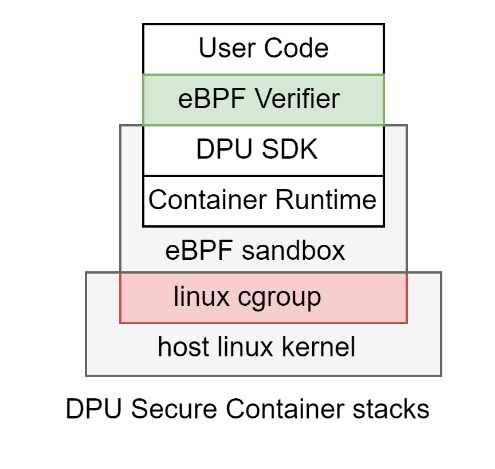
\includegraphics[width=0.4\textwidth]{figures/figure0}
 \label{fig:Overview-1}
 \caption{Overview}
\end{figure}



\subsection{研究目标和内容}
\ensection{Research objectives and content}
本论文的主要研究目标是通过优化Linux内核cgroup机制,提高Serverless环境下容器的并发启动性能;通过引入静态程序验证技术,保证Serverless平台中DPU资源的多租户安全隔离。具体内容包括:

优化cgroup机制:研究并优化Linux cgroup在高并发、大规模容器启动场景中的性能瓶颈,提高其在Serverless环境中的可扩展性和响应速度。
eBPF验证技术的应用:通过引入eBPF verifier等静态验证技术,确保Serverless平台中异构计算资源(如DPU)的安全隔离,避免不同租户间的资源竞争和安全问题。
通过以上研究,本论文旨在为异构计算平台下的Serverless架构提供高效、安全的容器应用加速技术,为下一代云计算平台的发展做出贡献。

\section{国内外研究现状}
\ensection{Research Progress Overview in Home and Abroad}
%\label{sec:***} 可标注label

国外学术界与工业界针对Serverless冷启动问题已展开多方面探索,主要集中在容器技术优化、虚拟化层轻量化与资源调度创新三个方向:

容器与镜像加速:微软提出基于并行化镜像构建的FAST-BUILD技术,通过文件级缓存复用机制减少容器构建时间 2;AWS采用分布式多级缓存的镜像分发策略,结合Block存储优化,缩短镜像拉取时延 2。此外,MIT团队开发的RemoteFork利用RDMA共享内存技术,将跨节点实例启动的数据拷贝延迟降至微秒级 3。
轻量级虚拟化:Google的gVisor通过用户态内核模拟实现安全容器隔离,启动时间压缩至毫秒级 2;斯坦福Catalyzer项目针对安全容器进行深度裁剪,结合预加载机制进一步降低初始化开销 2。
非容器运行时技术:剑桥大学提出基于WebAssembly(WASM)的Faasm框架,以进程级隔离替代容器虚拟化,在内存安全性与启动速度上取得平衡 3。
尽管上述技术显著优化了冷启动的部分环节,但仍存在以下局限:

cgroup并发瓶颈未解:现有研究多聚焦于容器运行时优化,但cgroup在高并发场景下的资源分配效率问题仍缺乏针对性设计 2;
虚拟化层冗余开销依存:即使轻量级容器(如Kata Containers)启动时间已优化至亚毫秒级,其内核加载与资源分配仍占用总延迟的30\%以上 3。
2. 国内研究动态
国内企业与研究机构在Serverless冷启动优化中侧重于镜像本地化与资源预配置:

镜像快速分发:阿里云提出基于树结构的跨节点镜像分发方案FaasNet,通过并行传输与增量更新技术将镜像分发效率提升40\% 2;华为云FunctionGraph采用Pod池化技术,通过预创建特化实例跳过镜像传输阶段,实现毫秒级实例启动 2 4。
运行时环境加速:字节跳动ByteFaaS平台引入本地代码缓存机制,结合动态链接库预加载技术,将Python函数启动时间降低33\% 3;华为云通过共享内存加速与依赖包预解压技术,将冷启动延迟压缩至10ms以内 4。
智能资源调度:腾讯云提出基于负载预测的动态缓存算法,通过机器学习模型预估实例需求,冷启动发生率降低60\% 3。
然而,国内研究仍面临挑战:

cgroup性能优化不足:现有方案依赖资源池化缓解压力,但未解决cgroup自身在高并发创建时的锁竞争与调度效率问题 2;
静态程序分析缺位:eBPF技术多用于网络性能优化(如Cilium),尚未与函数代码特征分析结合以替代虚拟化层 4。
3. 研究空白与突破方向
当前国内外研究呈现两大共性局限:

cgroup并发控制机制僵化:传统cgroup框架的任务调度策略难以应对突发性高密度函数实例创建需求,导致资源分配成为冷启动链路的性能瓶颈 2 3;
虚拟化层与函数逻辑割裂:现有优化多从“加速容器启动”角度切入,但未深入挖掘函数代码特性以绕过虚拟化层 3 4。
针对上述问题,本研究提出:

cgroup动态批量操作机制:借鉴无锁队列与异步资源分配策略,优化高并发场景下的控制平面性能(如单节点支持500+实例/秒的创建速率) 2;
eBPF驱动的函数静态分析:通过提取函数系统调用依赖与内存访问模式,预构建轻量化运行环境,实现无虚拟化层的“按需隔离” 3 4。
这一方向突破了传统优化路径,为Serverless冷启动问题提供了底层资源管理革新与函数逻辑感知的双重解决方案,有望推动边缘计算与实时AI推理等场景的规模化应用。


\section{本文主要内容和章节安排}
\ensection{Major Contents and Chapter Arrangement}

%\label{sec:features}



